\documentclass{beamer}

\usetheme{Madrid}


\usepackage{graphicx} 
\usepackage{enumerate}
\usepackage{amsmath,amssymb}
\usepackage{underscore}
\usepackage{multirow}
\usepackage{graphics}
\usepackage{multimedia}
\usepackage{hyperref}


\title{RMCS second minor}
\author{B.N.S.K. CHAITANYA \\
12MCMT02 }
\date{OCT 29, 2012}
\begin{document}

\begin{frame}[plain]
 \titlepage
\end{frame}

\begin{frame}
\frametitle{Mathematical formulas:}
\begin{equation}
\Re{z} =\frac{n\pi \dfrac{\theta +\psi}{2}}{
\left(\dfrac{\theta +\psi}{2}\right)^2 + \left( \dfrac{1}{2}
\log \left\lvert\dfrac{B}{A}\right\rvert\right)^2}.
\end{equation}

\begin{eqnarray}
{\cal B}(t,\omega) & \approx &
{1 \over 4\pi}
{\cal D}_tˆ2 W_{\bf S}(t, \omega)
{{{\scriptstyle \infty} \atop
{\displaystyle \int \! \int \!
}}\atop {\scriptstyle -\infty}}
t_1ˆ2
\phi(t_1,\omega_1) \, dt_1 d\omega_1
\nonumber \\
&& +
{1 \over 4\pi}
{\cal D}_\omegaˆ2 W_{\bf S}(t, \omega)
{{{\scriptstyle \infty} \atop
{\displaystyle \int \! \int \!
}}\atop {\scriptstyle -\infty}}
\omega_1ˆ2
\phi(t_1,\omega_1) \, dt_1 \, d\omega_1.
\label{F4}
\end{eqnarray}

\begin{eqnarray}
{\cal M}ˆ2(\hat{\theta},\theta) &=& E[(\hat{\theta} - \theta)ˆ2]
\nonumber \\
{\cal M}ˆ2(\hat{\theta},\theta) &=& {\rm var}ˆ2(\hat{\theta}) +
{\cal B}ˆ2(\hat{\theta}).
\end{eqnarray}
\end{frame}

\begin{frame}
\frametitle{Slide containing a table of marks of the student}
\begin{table}[ht]
\centering
\begin{tabular}{|l|l|l|l|l|}
 \hline
 \multicolumn{5}{|c|}{\textbf{Marks secured by the students}} \\
 \hline
   \emph{RollNo.} & \emph{Name} & \emph{M1  M2  Tot} & \emph{Major} & \emph{Total(100)} \\ \hline
 \hline
01 & Chris Nihar & 19   13   32 & 50 & 82  \\ 
 \hline
02 & B.N.S.K. Chaitanya & 18  10  28 & 50 & 78   \\
\hline
03 & Satish & 18 15 33 & 50 & 83 \\
\hline
\end{tabular}
\caption{This table contains the marks of the students}
\label{tab:Marks of students}
\end{table}
\end{frame}

\begin{frame}
\frametitle{Slide containing the photograph and some facts about my favourite mathematician...}
\begin{columns}[c]
\column{5cm}
\textbf {Evariste Galois}
\framebox{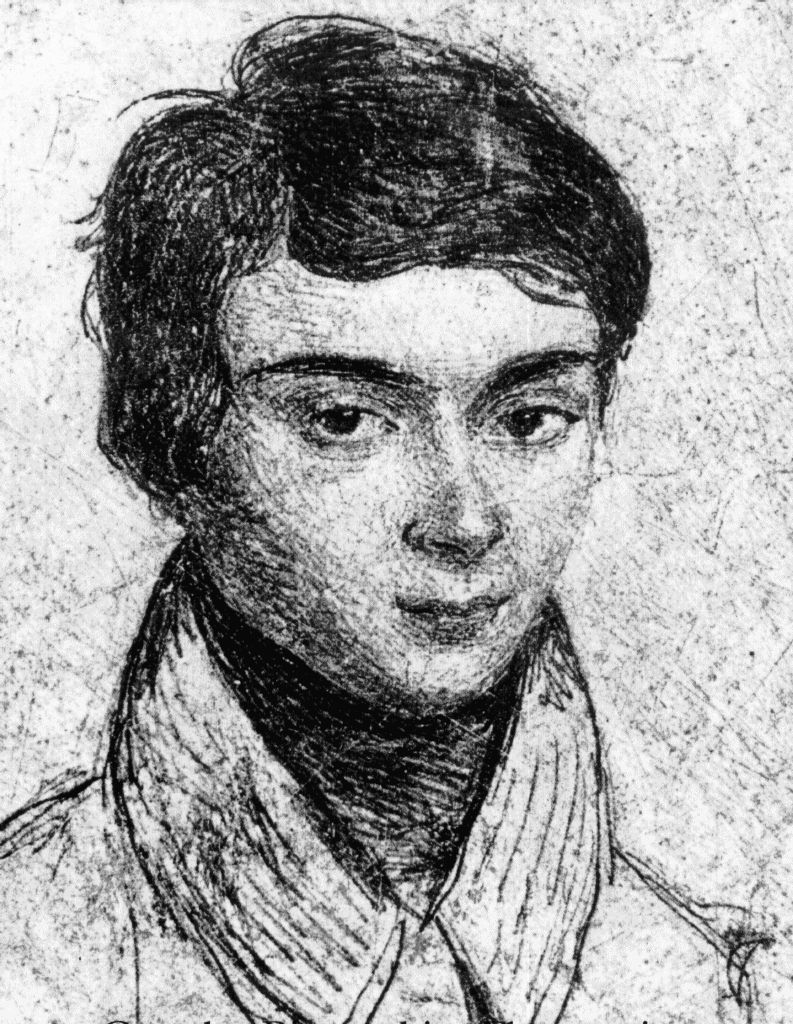
\includegraphics[width=3cm]{galois.jpg}}
\column{7cm}
\Large Evariste Galois\\
 \normalsize
\textbf Some facts:
\begin{enumerate}
\item 25 October 1811-31 May 1832\\
\item During his teens itself,infact at the age of 21,the night before he died,he wrote down all the theory which is now being called the "Galois Theory".\\   
\item This means he created a whole new branch of Mathematics overnight literally!!!\\
\end{enumerate}
\end{columns}
\end{frame}

\begin{frame}
\frametitle{My Other Favourite mathematicians..}
\begin{itemize}
\item  
\begin{block}{Leonhard Euler}
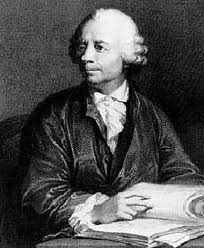
\includegraphics[scale=0.2]{euler.jpg}
      Infinitesimal Calculus,Graph Theory,Fluid dynamics,geometry,optics,etc.!!!!
\end{block}
\item  
\begin{block}{Srinivasa Ramanujam}
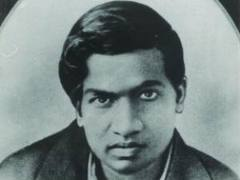
\includegraphics[scale=0.2]{ramanujam.jpg}
      Trigonometry,mathematical analysis,continued fractions,Number-theory,infinite series,etc.!!!!
\end{block}
\end{itemize}
\end{frame}



\end{document}

